\documentclass[10pt,preprint]{sigplanconf}
\usepackage{times}
\usepackage{datetime}
\usepackage{url}
\usepackage{hyperref}
\usepackage{amssymb}

% TODO: remove draft
\usepackage{graphicx}

\conferenceinfo{SOSP'17}{October 29--31, 2017, Shanghai, China}
\copyrightyear{2017}


% These only appear when the 'preprint' option is specified.
% Enabling these will cause the first page of the document to fail the
% format check on HotCRP :-(
% TODO: remove before submitting
\titlebanner{Under submission to SOSP 2017 - do not cite or distribute}
\preprintfooter{Draft of {\currenttime}, \today{}}

% No date in title area.
\date{}

% Paper number and no. of pages as author
% TODO: Replace 'XX' with your paper number (assigned when you register abstract)
% TODO: Replace 'NN' with actual number of pages.
\authorinfo{Paper \textbf{\#XX}}{NN pages}

% Actual document begins below.
\begin{document}

\title{The case for [dynamically scalable parallelism]}
\maketitle

\begin{abstract}
In recent years, economic and physical realities have pushed both chip designers and application developers to rely increasingly on parallelism to satisfy performance demands \cite{mack2011fifty}. However, there is no free lunch. Even after an application developer has wrestled with several target architectures, she still does not know what resources the application will get at runtime. Often, it is easier to over-provision units of execution and hope for the best. Yet even mild contention can drastically reduce overall system throughput and wall-clock execution times of individual applications. On the other hand, under-provisioning units of execution means leaving resources unused and falling short of performance potential. In this paper, we show that by selectively and dynamically changing application parallelism, we can avoid both pitfalls [in some way].

Stronger guarantees from scheduler to application (monitor actual resource utilization). Insights from application to scheduler (e.g., some information about app?).

\end{abstract}


\section{Questions}
\begin{itemize}
  \item How do developers typically provision number of threads? How do they determine the maximum?
\end{itemize}

\section{To do}
\begin{itemize}
  \item DS Paper outline
  \item MS AC Understand difference in performance for different levels of parallelism
  \item [\checkmark] Understand Intel TBB
  \item Design interface between library and coordinator
  \item Implement and integrate coordinator with library
  \item Integrate library into applications
  \begin{itemize}
    \item http://wiki.cs.princeton.edu/index.php/PARSEC
  \end{itemize}
  \item Evaluations
  \item Run ./bin/todo to find remaining todos in tex files
\end{itemize}

\section{Introduction}
Parallelism and cotenancy are the future. However, people program as though there is no cotenancy. This causes performance problems. Today, people statically partition. Utilization is not great and you don't get perfect isolation anyway.
\subsection*{Parallelism and cotenancy are here to stay}
\begin{itemize}
  \item Increasing number of cores \cite{baumann2009multikernel}
  \item As a result, application developers must think about parallelism to get performance
  \item Cloud becoming increasingly popular; run many containers / VMs on a single host and want performance guarantees for tenants (sophisticated orchestration / scheduling)
\end{itemize}
\subsection*{Developers / OS have digested parallelism, but not cotenancy}
\begin{itemize}
  \item Developers: assume have full machine (over-provision) because not easy to know what resources we have.
  \item OS: schedule individual threads (Linux). Some control with cgroups to coordinate groups of threads.
\end{itemize}
\subsection*{What's are the issues}
\begin{itemize}
  \item Over-provisioning may low utilization on many core
  \item CPU share and quota (cgroup) not enough; need to change parallelism of applications to affect utilization
  \item [TODO: INSERT SMALL EXAMPLE] since different applications have different overheads / slow-down in total CPU time
\end{itemize}
\subsection*{Contributions}
\begin{itemize}
  \item Observe that dynamically scaling parallelism can improve system performance (throughput, latency)
  \item Thread library that can dynamically scale application parallelism
  \item User-level coordinator to determine appropriate level of parallelism for registered applications
\end{itemize}

% \section{Motivation for a dynamic parallelism}
\begin{itemize}
  \item Many cores are here to stay. Need more automated methods to take advantage of. \cite{baumann2009multikernel}
  \item OS schedulers already quite complex. Must serve many masters; hard to make changes without harming certain workloads. Don't want to change the kernel if we can improve performance in user space \cite{lozi2016linux}
  \item Applications are being increasingly run in containers / VMs on a single host
  \item Centralized schedulers in distributed systems struggle to scale \cite{ousterhout2013sparrow}
\end{itemize}

\section{Performance of parallel programs}

Note: will cover PARSEC/Splash2 in more detail in later section \cite{bienia2011benchmarking} \cite{bienia2008parsec} \cite{bienia2012characteristics}

\subsection{Performance without contention}

% TODO: replace with speed-up graph
\begin{figure}
\centering
  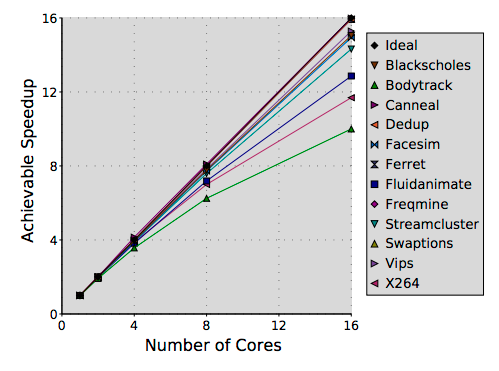
\includegraphics[width=8cm,height=4cm]{fig/speed-up.png}
  \caption{PLACEHOLDER: Wall-clock speed-up time. Upper bound for speedup of PARSEC workloads with input set simlarge based on instruction count. Limitations are caused by serial sections, growing parallelization overhead and redundant computations.}
  \label{fig:speed-up}
\end{figure}

% TODO: replace with slow-down total cpu time graph
\begin{figure}
\centering
  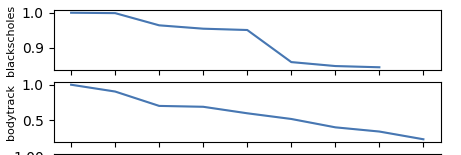
\includegraphics[width=8cm,height=4cm]{fig/slow-down.png}
  \caption{PLACEHOLDER: Although applications typically enjoy wall-clock speed-up times when they use more threads, often see corresponding increase in total CPU time [this graph might be confusing since we're talking about increase in total CPU time, but curve is going down]}
  \label{fig:slow-down}
\end{figure}

\begin{itemize}
  \item speed-up curve (see Figure \ref{fig:speed-up})
  \item slow-down curve (see Figure \ref{fig:slow-down})
\end{itemize}

\subsection{Performance under contention}

% TODO: replace with nicer figure for contention same
% TODO: need figure with mixed applications
\begin{figure}
\centering
  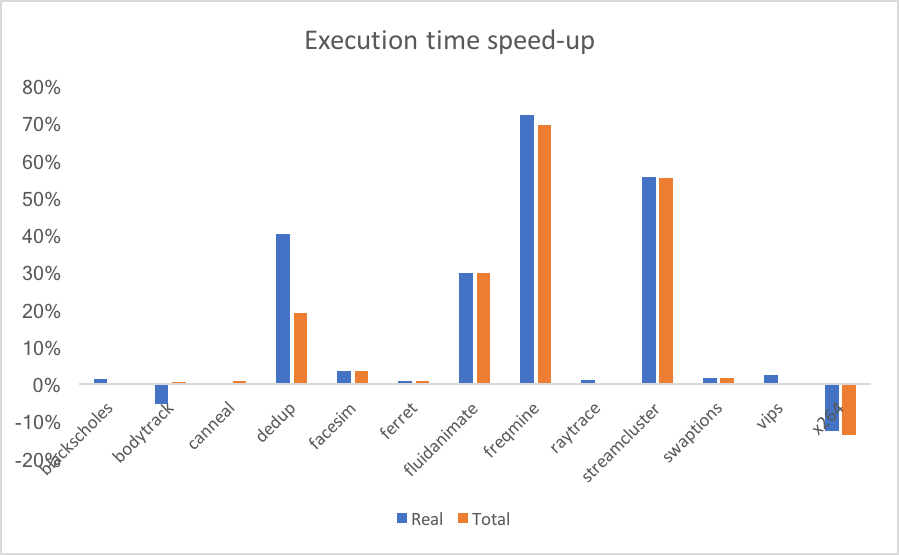
\includegraphics[width=8cm,height=4cm]{fig/contention-same.png}
  \caption{PLACEHOLDER: How groups of applications (same or mixed (need this fig)) do under contention at varying \# of threads}
  \label{fig:contention-same}
\end{figure}

\begin{itemize}
  \item same application (see Figure \ref{fig:contention-same})
  \item mixed group of applications (see Figure [])
\end{itemize}

\subsection{Reasons for contention}
\begin{itemize}
  \item thread contention (manny runnable threads, but divided work up into small pieces; not overlapping well with i/o)
  \item lock contention (why would this be exacerbated under contention?)
  \item other resource contention
\end{itemize}

\textbf{Classes of application behavior}
\begin{itemize}
  \item Big improvement from reducing parallelism (dedup, facesim, freqmine, streamcluster)
  \item Slight improvement from reducing parallelism
  \item Performance hit from reducing parallelism (x264)
\end{itemize}

\subsection{Common strategies for dealing with unknown resources}
TODO: maybe delete this section?
\begin{itemize}
  \item Overprovision number of threads and hope for the best. But this can cause problems (e.g., lock or resource contention)
\end{itemize}

\section{Determining contention and who should change parallelism}
TODO: change section title

TODO: maybe this shouldn't be its own section

\subsection{System metrics for determining contention}
\begin{itemize}
  \item \# of runnable threads
  \item CPU utilization
\end{itemize}

\subsection{Application metrics for determining candidates for parallelism scaling}

\section{Design}
Not sufficient to set parallelism just at application start, need to scale up and down. Machine load may change over time. Application requirements may change within a single run

\subsection{Mechanism for communicating}
\begin{enumerate}
  \item Use kernel memory (must modify kernel)
  \item User space
\end{enumerate}

\subsection{Thread library}
Similar to Intel Thread Building Blocks \cite{reinders2007intel}, but dynamically scale number of workers across applications, rather than just across workers
\begin{itemize}
  \item Types of blocks: iterative / non-iterative parallelized operations
  \item DAG
  \item Unstructured
\end{itemize}

Global queue vs. fixed partition + work stealing

Min/max number of threads set by application developer

I/O and CPU pools treated differently in most libs

\begin{figure}
\centering
  \includegraphics[width=8cm,height=4cm]{overhead.png}
  \caption{What is performance overhead of thread library over pthreads?}
\end{figure}
\subsection{Driver application}
Track CPU utilization by application (any other metrics?)
Change target parallelism (how to decide, when to decide, how much to change by, which to change)
Change CPU share or quota
\subsection{Client applications}

\section{Benchmark applications}

\begin{itemize}
  \item TODO: do we want a single large application (e.g., provisioned for KNL, but running on much smaller VM for some reason)?
  \item TODO: What about an unstructured application (e.g., web server)?
  \item TODO: What about long-lived application (e.g., streaming)? We can probably simluate this via streamcluster
\end{itemize}

\subsection{PARSEC}

\subsection{SPLASH-2}
TODO: maybe leave this out given timing

% \section{Implementation}

\section{Evaluation}
\subsection{Workloads}
Different classes of applications. Mixture of applications.

Should we have single large application?

How should we handle unstructured parallel programs (e.g., web server?)

\subsection{Comparison with other thread libraries}
OS (pthreads), OpenMP, Intel TBB
\subsection{Varying guarantees (CPU share / quota)}

\subsection{Various machines}

\section{Related work}
\subsection{Parallel programming libraries}
\subsection{Application / OS interface}
\begin{itemize}
  \item Intel TBB \cite{contreras2008characterizing}
  \begin{itemize}
    \item https://software.intel.com/en-us/blogs/2007/08/13/threading-building-blocks-scheduling-and-task-stealing-introduction
    \item https://software.intel.com/en-us/node/506294
  \end{itemize}
  \item Microsoft PPL
  \begin{itemize}
    \item https://msdn.microsoft.com/en-us/library/gg663539.aspx
  \end{itemize}
  \item Scheduler activations \cite{anderson1992scheduler}
  \item Cilk \cite{blumofe1995cilk}
  \item Charm++
  \item OpenMP
  \item Chare
  \item Multikernel
  \item Exokernel
  \item Hierarchical schedulers
  \item Cache-aware / contention-aware / numa-aware schedulers
  \item Arachne
  \item Capriccio
  \item Wasted cores
\end{itemize}

\section{Discussion and future work}
Whatever we didn't finish

Making a case

Don't claim optimal


\section*{Acknowledgements}

\bibliography{citations}{}
\bibliographystyle{acm}

\end{document}
